\chapter{Higher order AGP as a cost function}\label{chap:7_higher_order_agp}

\section{Return to two-spin annealing}

Hey there's lots of cool stuff to see here! Check out Appendix \ref{app:higher_order_AGP} for more nice plots and things. I might just keep the stuff in Fig.~\ref{fig:two_spin_higher_order} for now to keep it focused.

\begin{figure}[h]
    \centering
    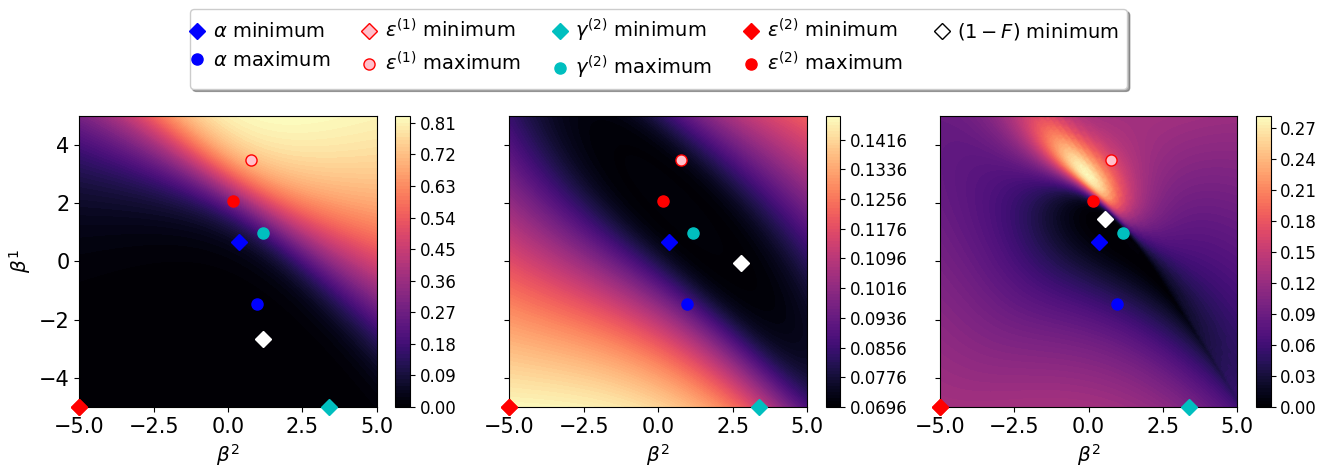
\includegraphics[width=\linewidth]{images/2spin_Integrals_scaled_by_norm_final.png} \caption[Two-spin annealing fidelity contour plots]{Current placeholder for final figure. (a) Only first order CD is applied. (b) only $\sz\sy, \sy\sz$ terms are applied. (c) All second-order terms are applied ($\sz\sy, \sy\sz$, $\sx\sy, \sy\sx$).}\label{fig:two_spin_higher_order}
\end{figure}

\section{GHZ states, fidelity and entanglement}

\begin{figure}[t]
    \centering
    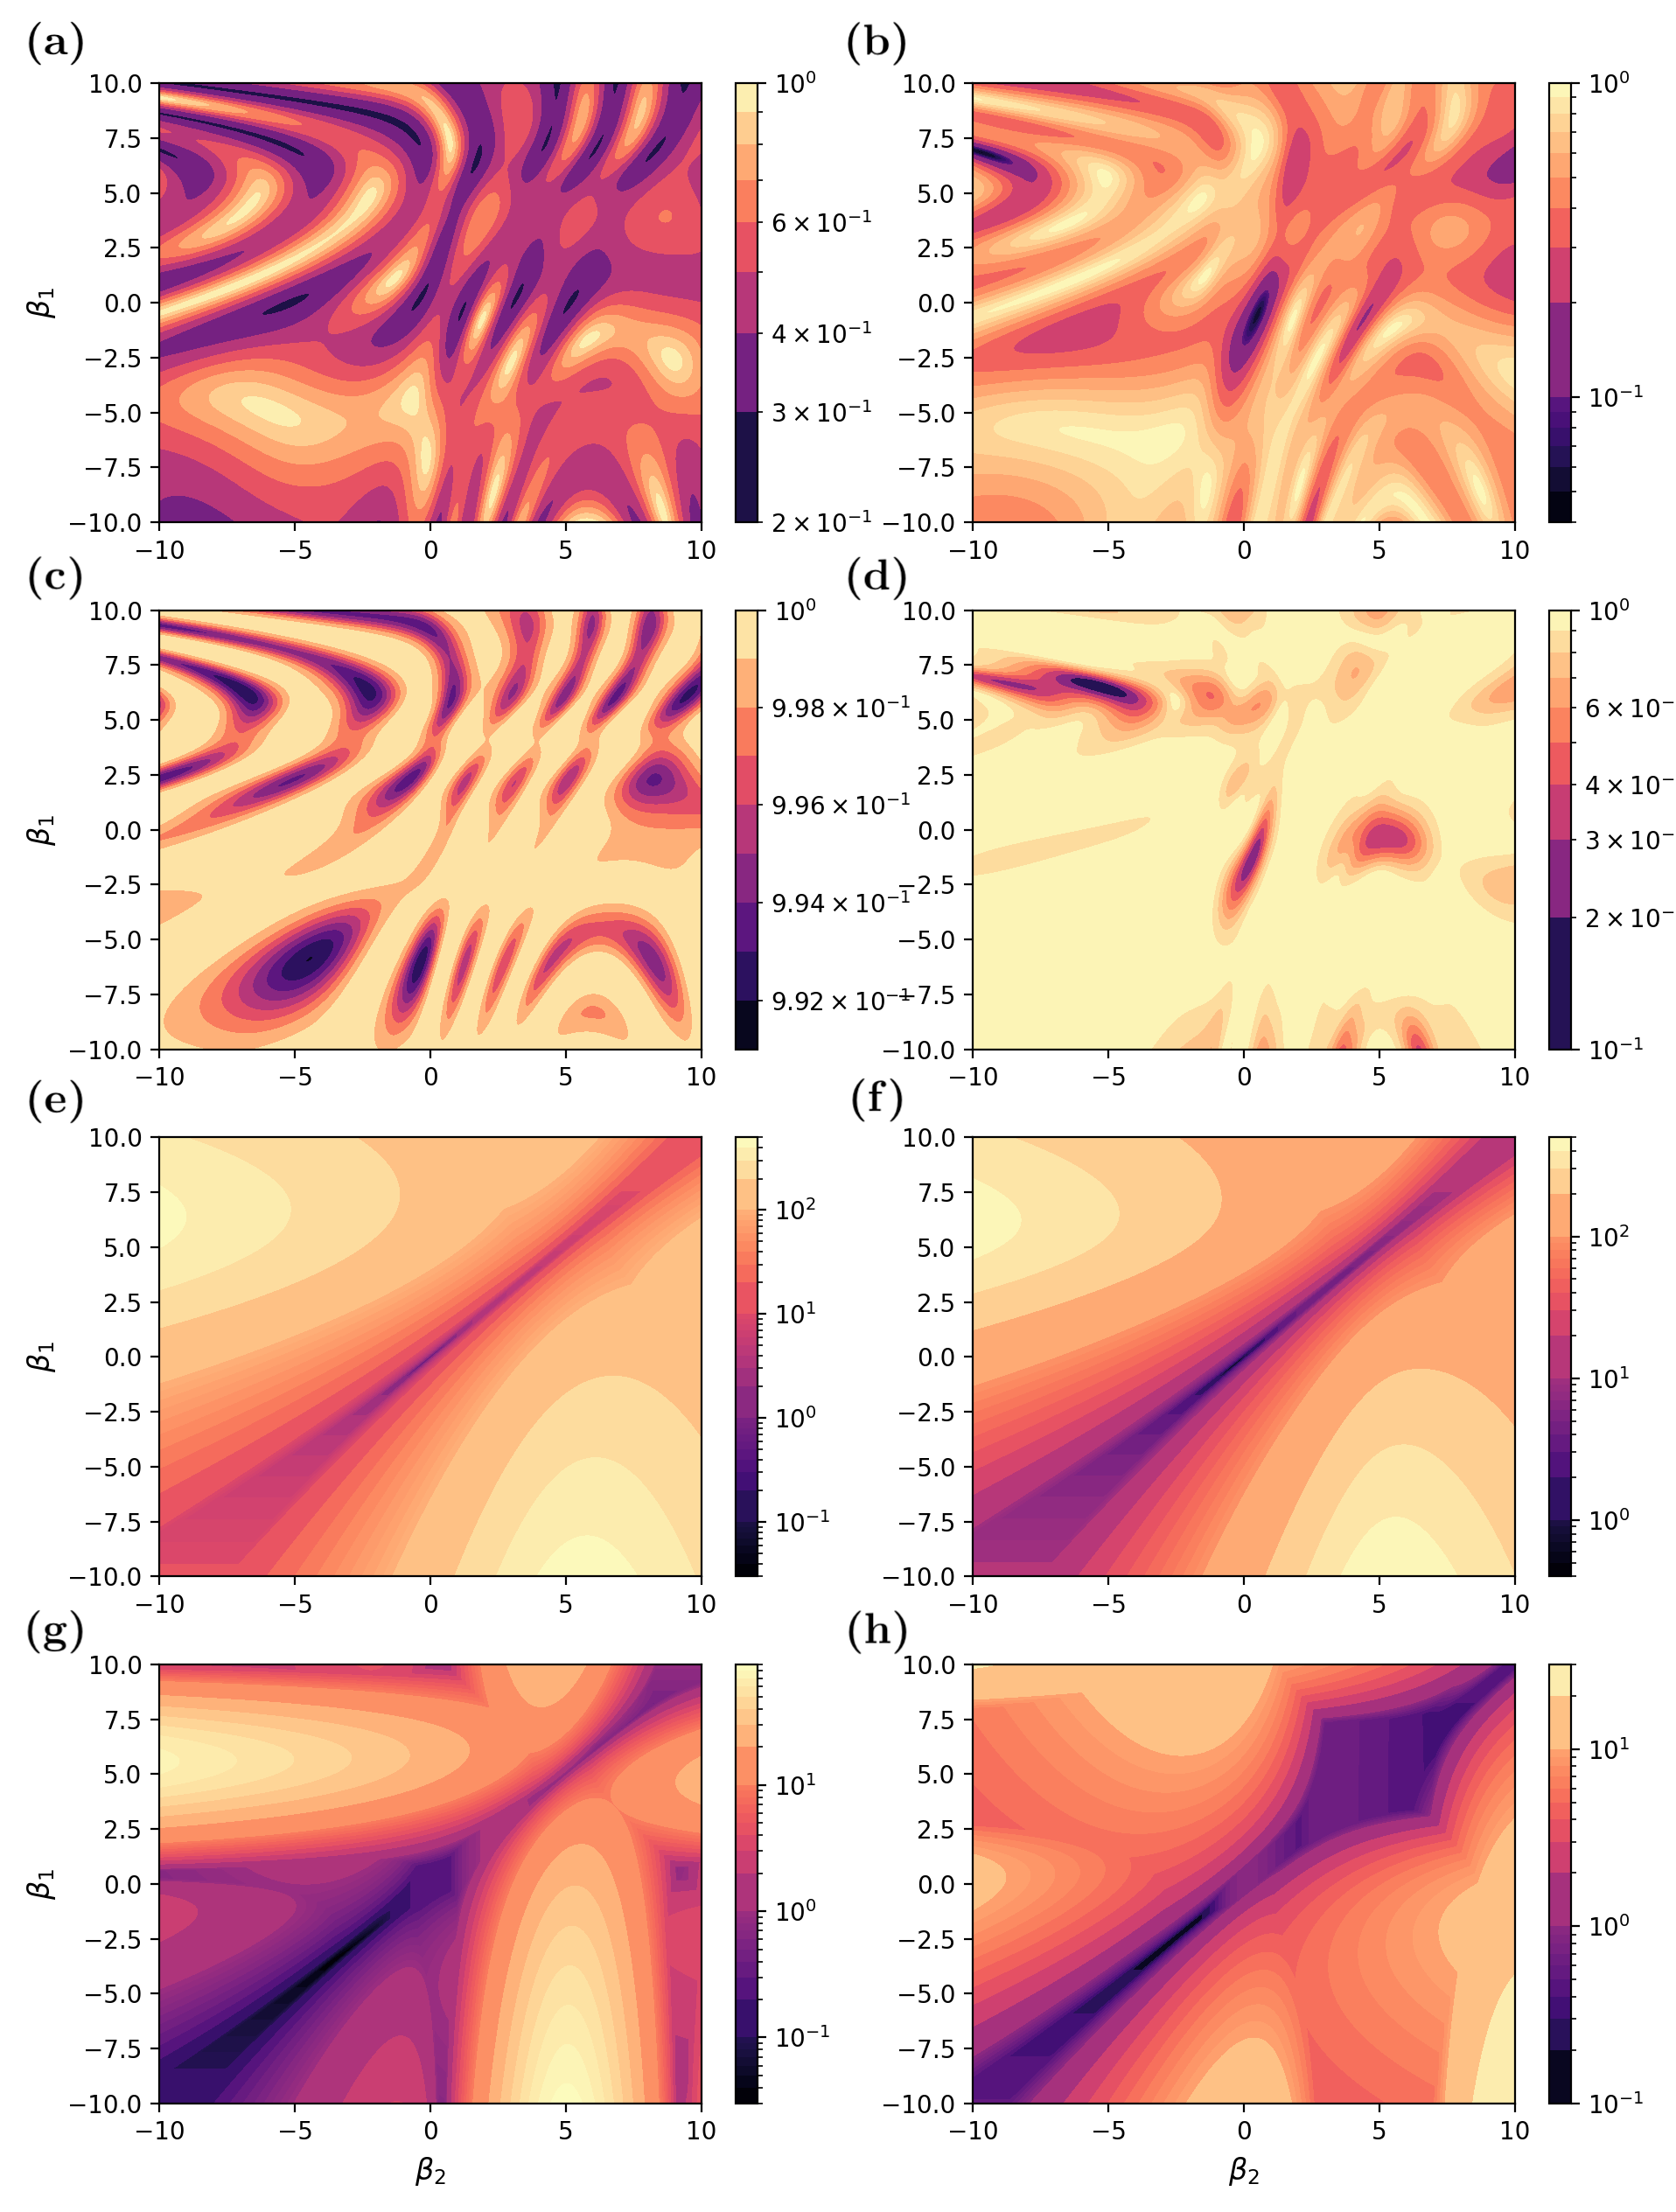
\includegraphics[width=\linewidth]{images/ghz_contour_plots.png} \caption[Contour plots of cost function landscapes for GHZ state preparation in frustrated spin systems.]{Contour plots, $\tau = 0.1 J^{-1}$, \acrref{GRAPE} for parameters $\beta_1$ and $\beta_2$. (a) FO CD infidelity, (b) SO CD infidelity, (c) FO CD $1 - T_3$, (d) SO CD $1 - T_3$, (e) FO CD amps ($\alpha$), (f) SO CD amps ($\alpha$) (g) SO CD amps ($\gamma$) (h) SO CD amps ($\zeta$)}\label{fig:two_spin_higher_order}
\end{figure}